% TODO: images are on counted
\section{ЗАДАЧІ МАРКЕТИНГОВОЇ РОЗВІДКИ ТА МОДЕЛЮВАННЯ МАРКЕТИНГОВИХ КАНАЛІВ}
% Ми не створюємо канал як такий. Метою роботи є маркетингове прогнозування 
% шляхом моделювання маркетингового каналу.
%
% TODO: можливо, заголовок треба буде змінити
% TODO: додати новий сорець
\subsection{Основні проблемі розробки програмних систем}
\subsubsection{Основні поняття}
% TODO: програмна інженерія
% TODO: програмне забезпечення
% TODO: системна вимога
% TODO: програмний засіб
% TODO: системні вимоги
% TODO: проблемна область  
\subsubsection{Необхідність створення ПС}
\subsubsection{Процес розробки ПЗ}
% TODO: МЖЦ, методології
\subsubsection{Нотація, що використовується}
% TODO: UML, IDEF*

\subsection{Маркетингові інформаційні системи}
\subsubsection{Необхідність створення МІС}
%    Компанії зростають, роль маркетологів зростає.
Кожна зростаюча компанія коли-небудь зтикається з необхідністю розробки маркетингової стратегії та планування маркетингової діяльності відповідно до розробленої стратегії. Маркетингова стратегія --- це процес, що дозволяє компанії досягати росту продажів та сталих конкурентних переваг, концентруючи ресурси тільки на оптимальних можливостях\cite{baker}. За рішення про вибір та використання ринкових можливостей компанії відповідає маркетинговий підрозділ компанії. 
 
Для підтримки прийняття рішень, маркетологи повинні бути забезпечені постійним доступом до точної та актуальної інформації про клієнтів, продажі, конкурентів тощо. В процесі збору цієї інформації виникають проблеми, що пов’язані з ростом компанії, тобто, з масштабуванням бізнес-процесів: зростають об’єми інформації, зростає час, необхідний на обробку та аналіз, зростають витрати на зберігання. Для вирішення цих проблем використовують системи підтримки прийняття рішень, до яких відносять і маркетингові інформаційні системи. Маркетингова інформаційна система або МІС (англ. {\it marketing information system, MkIS}) --- це сукупність людей та систем, що виконують процедури збору, сортування, аналізу та оцінки інформації для підтримки прийняття маркетингових рішень \cite{kotler14}. МІС може входити до складу більш загальної системи підтримки прийняття керівних рішень, EIS (англ. {\it executive information system}).
    
\subsubsection{Проблеми МІС}
%    MIS складається з трьох частин:
Маркетингова інформаційна система складається з трьох частин\cite{kotler14}:
\begin{itemize}
\item {\it Внутрішній облік.} Системи внутрішнього обліку збирають інформацію про продажі на клієнтів, це можуть бути CRM та ERP системи.
\item {\it Аналіз та дослідження.} Це люди та спеціалізовані системи, що займаються аналізом ретроспективної та поточної інформації. Процес аналізу автоматизують за допомогою OLAP-систем та data mining систем.
\item {\it Маркетингова розвідка.} Це процедури, за допомогою яких маркетологи збирають повсякденну інформацію про події та тенденції, що є на ринку. 
\end{itemize}
% TODO: схему в иллюстрации и слайди!
На основні ретроспективни даних, що були зібрані системами внутрішнього обліку, аналітики роблять висновки про наявні результати, помилки, що були допущені. Але найбільший інтерес викликають системи маркетингової розвідки, за допомогою яких	 .   
%    Внутрішнє -- це класи систем ERP та CRM
%    Аналіз -- це вирокистання ретроспективних даних, зібраних внутрішнім обліком. Роблять аналітики
%    Маркетингова розвідка -- це..., що має на увазі: корпоративна/конкурентна розвідка
%    Проблема: відсутня система корпоративної розвідки ситуації на ринку.
%    
% \subsubsection{Корпоративна розвідка}
%    Корпоративна розвідка здійснюється наступними методами: ...
%    Пропонується робити розвідку шляхом моделювання маркетингового каналу.
%

% TODO: що це таке, навіщо воно потрібно, складові частини та їх призначення, 4Р
\begin{stdfigure}
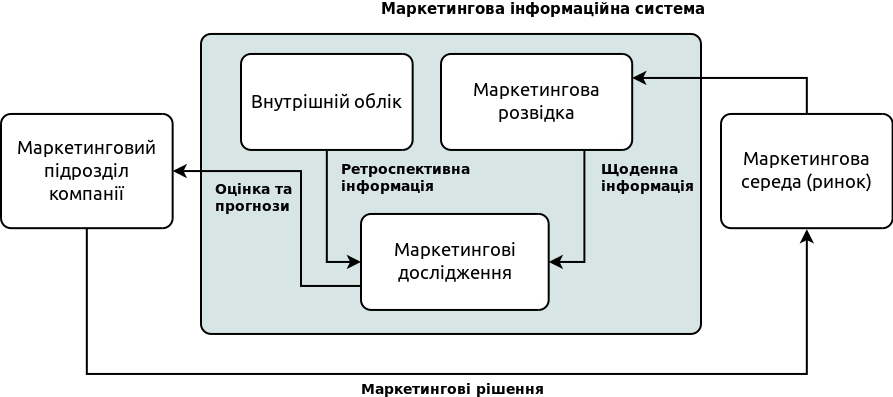
\includegraphics[width=6in]{images/mis_structure.png}
\caption{Структура МІС}
\label{fig:mis_structure}
\end{stdfigure}
 
Маркетингова інформаційна система складається з трьох частин (див. рис. \ref{fig:mis_structure}): 
\begin{longEnumerate}
\item Внутрішній облік. Це звітність з продажів, замовлень, цін, доставок і т.д., яка забезпечується системами класу CRM та ERP;
\item Маркетингові дослідження. Це системи аналізу даних: OLAP-системи та data mining системи;
\item Маркетингова розвідка. Це постійний збір інформації про ринок, клієнтів на конкурентів, що дозволяє прогнозувати ситуацію на ринку.
\end{longEnumerate}

\subsubsection{Маркетингова розвідка}
% TODO: Що то, нащо треба, як це робиться (моделювання, дослідження, etc), огляд наявних систем
% Це збір, ... інформації, що допомагає є основною для маркетингового дослідження: допомагає приймати рішення та прогнозувати ринок.
% Робиться ось так: ...
% Пропонується моделювати маркетинговий канал (дати визначення) для того, що перспективну інформацію.

\subsubsection{Бізнес-ігри}
% TODO: що таке бізнес-ігри, навіщо вони потрібні і як реалізються

\subsection{Постановка задачі}
\subsubsection{Моделювання маркетингового каналу}
%TODO: що таке концепція маркетингового каналу, основні момент структури та керування каналом.
% TODO: постановка задачі моделювання ()

\subsubsection{Вимоги до програмного забезпечення}